\documentclass{article}
\usepackage[utf8]{inputenc}

\title{EE2703 Week 7}
\author{Anand Uday Gokhale Roll Number : EE17B158 }
\date{March 2019}


\usepackage{natbib}
\usepackage{graphicx}
\usepackage{amsmath}
\usepackage{listings}

\begin{document}

\maketitle

\section{Introduction}
This week's assignment involves the analysis of filters using laplace transforms. Python's symbolic solving library, sympy is a tool we use in the process to handle our requirements in solving Modified Nodal Analysis  equations. Besides this the library also includes useful classes to handle the simulation and response to inputs.

Coupled with scipy's signal module, we are able to analyse both High pass and low pass filters, both second order, realised using a single op amp

\section{Assignment}
\subsection{Low pass Filter}
The low pass filter we use gives the following matrix after simplification of Modified Nodal Equations.
\newline
$\begin{bmatrix}
    0   & 0 & 1  & -1/G \\
    \frac{-1}{sR_2C_2}  & 1 & 0 & 0\\
    0  & -G & G & 1 \\
    \frac{-1}{R_1} - \frac{1}{R_2} - s*C_1 & \frac{1}{R_2} & 0 & sC_1
\end{bmatrix}$
$\begin{bmatrix}
    V_1\\
    V_p\\
    V_m \\
    V_o
\end{bmatrix}$
=
$\begin{bmatrix}
    0 \\
    0 \\
    0 \\
    \frac{-V_i(s)}{R_1} \\
    
\end{bmatrix}$
\lstset{language=Python}
\lstset{frame=lines}
\lstset{label={lst:code_direct}}
\lstset{basicstyle=\footnotesize}
\newline
\newline
\begin{lstlisting}
def lowpass(R1,R2,C1,C2,G,Vi):
    s=  sympy.symbols("s")
    A = sympy.Matrix([[0,0,1,-1/G],\
            [-1/(1+s*R2*C2),1,0,0],\
            [0,-G,G,1],\
            [-1/R1-1/R2-s*C1,1/R2,0,s*C1]])
    b=  sympy.Matrix([0,0,0,-Vi/R1])
    V = A.inv()*b
    return A,b,V
\end{lstlisting}
The magnitude bode plot for the filter looks like:
\begin{figure}[h!]
\centering
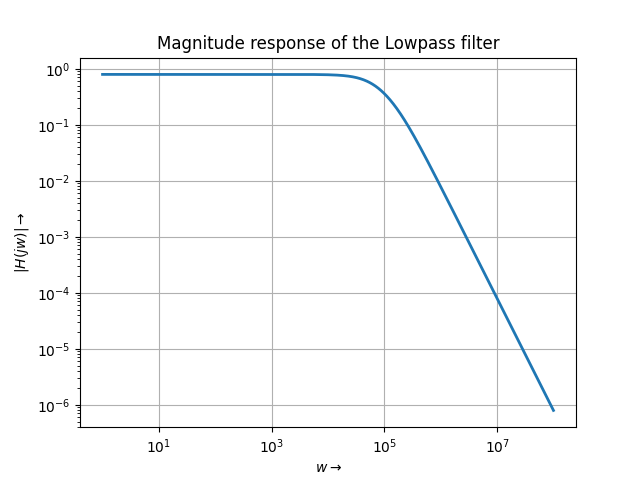
\includegraphics[scale=0.6]{Figure_1.png}
\caption{Lowpass filter magnitude response}
\label{fig:Lowpass filter magnitude response}
\end{figure}

\begin{figure}[h!]
	\centering
	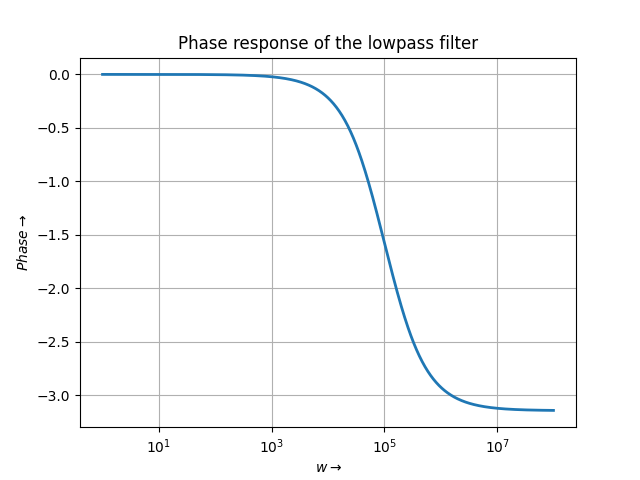
\includegraphics[scale=0.6]{Figure_2.png}
	\caption{Lowpass filter magnitude response}
	\label{fig:Lowpass filter magnitude response}
\end{figure}


The unit step response for the low pass filter:


\begin{lstlisting}
	def symToTransferFn(Y):
	Y = sympy.expand(sympy.simplify(Y))
	n,d = sympy.fraction(Y)
	n,d = sympy.Poly(n,s), sympy.Poly(d,s)
	num,den = n.all_coeffs(), d.all_coeffs()
	num,den = [float(f) for f in num], [float(f) for f in den]
	return num,den
	
	def stepresponse(Y):
	num,den = symToTransferFn(Y)
	den.append(0)
	H = sp.lti(num,den)
	t,y=sp.impulse(H,T = np.linspace(0,1e-3,10000))
	plt.plot(t,y)
	plt.show() 
	return
	s =  sympy.symbols("s")
	A,b,V=lowpass(10000,10000,1e-9,1e-9,1.586,1)
	stepresponse(V[3])
\end{lstlisting}


\begin{figure}[h!]
	\centering
	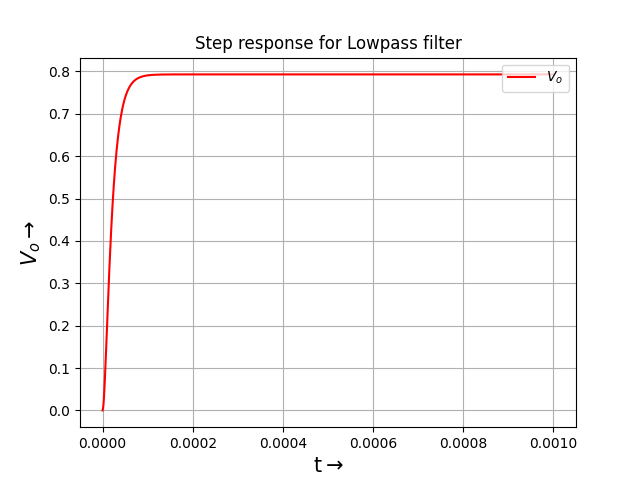
\includegraphics[scale=0.6]{Figure_3}
	\caption{System Response with Decay = 0.5}
	\label{fig:System Response with Decay = 0.5}
\end{figure}


\subsection{Response of Lowpass Filter to mixed frequency sinusoid}
We now see what happens with a input as a sum of sinusoids.
\begin{figure}[h!]
	\centering
	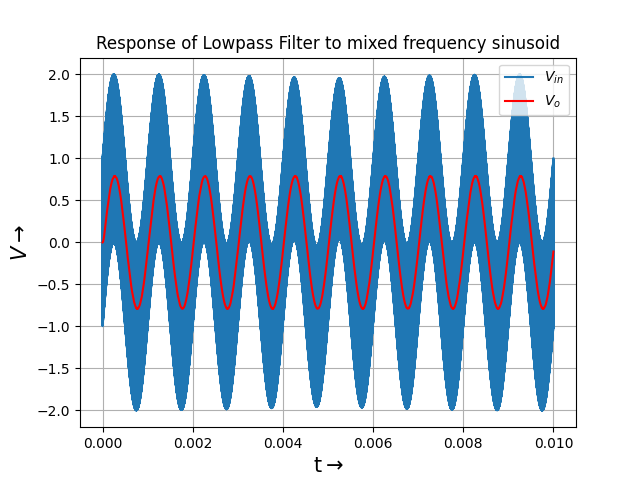
\includegraphics[scale=0.6]{Figure_4}
	\caption{Sum of sinusoids}
	\label{fig:System Response with Decay = 0.05}
\end{figure}

\begin{lstlisting}
	def inputs(t):
	return (np.sin(2000*np.pi*t)+np.cos(2e6*np.pi*t))
	
	def inp_reponse(Y,inp=inputs,tlim=1e-3):
	num,den = symToTransferFn(Y)
	H = sp.lti(num,den)
	t = np.linspace(0,tlim,100000)
	t,y,svec = sp.lsim(H,inp(t),t)
	plt.plot(t,y)
	plt.show() 
	return
\end{lstlisting}

We notice that the high frequency part has been attenuated.



\clearpage
\subsection{High pass Filter}

The high pass filter we use gives the following matrix after simplification of Modified Nodal Equations.
\newline

$\begin{bmatrix}
    0   & -1 & 0  & 1/G \\
    \frac{s*C_2*R_3}{1+s*C_2*R_3}  & 0 & -1 & 0\\
    0  & G & -G & 1 \\
    -s*C_2 - \frac{1}{R_1} - s*C_1 & 0 & s*C_2 & \frac{1}{R_1}
\end{bmatrix}$
$\begin{bmatrix}
    V_1\\
    V_p\\
    V_m \\
    V_o
\end{bmatrix}$
=
$\begin{bmatrix}
    0 \\
    0 \\
    0 \\
    -V_i(s)*s*C_1 \\
    
\end{bmatrix}$
\newline
\newline
\begin{lstlisting}
def highpass(R1,R3,C1,C2,G,Vi):
    s=  sympy.symbols("s")
    A=sympy.Matrix([[0,-1,0,1/G],
        [s*C2*R3/(s*C2*R3+1),0,-1,0],
        [0,G,-G,1],
        [-s*C2-1/R1-s*C1,0,s*C2,1/R1]])
    b=sympy.Matrix([0,0,0,-Vi*s*C1])
    V=A.inv()*b

    return (A,b,V)
\end{lstlisting}

The magnitude bode plot for the filter looks like:
\begin{figure}[h!]
\centering
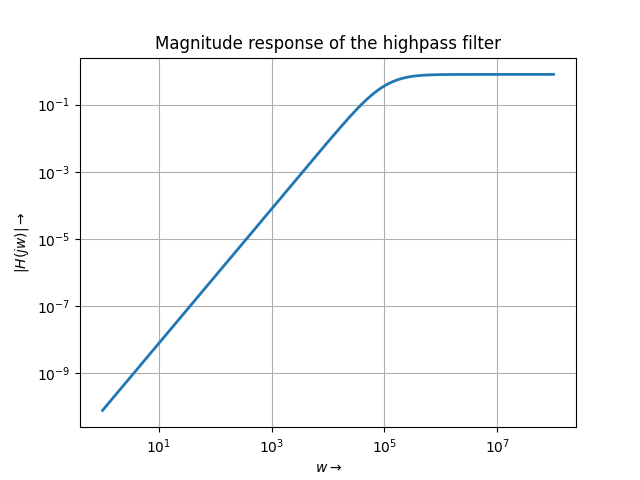
\includegraphics[scale=0.6]{Figure_5.png}
\caption{High pass filter magnitude response}
\label{fig:High pass filter magnitude response}
\end{figure}
\begin{figure}[h!]
	\centering
	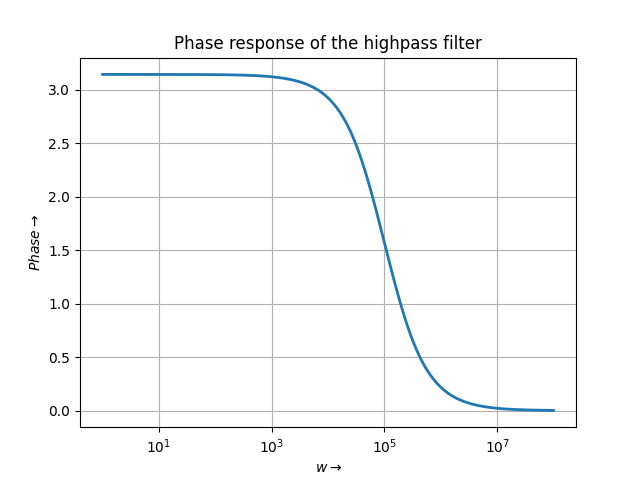
\includegraphics[scale=0.6]{Figure_6.png}
	\caption{High pass filter magnitude response}
	\label{fig:High pass filter magnitude response}
\end{figure}



\clearpage


\subsection{Response of Highpass filter to a damped sinusoid}

\subsubsection{Low frequency damped sinusoid}
The High frequency damping sinusoid is given by:
\begin{equation}
	f(t) = cos(10^3t)*e^{-1000t}
\end{equation}
It is expected that it will be fully attenuated by the high pass filter while it will pass through the Low pass filter with almost no change.
\begin{figure}[h!]
	\centering
	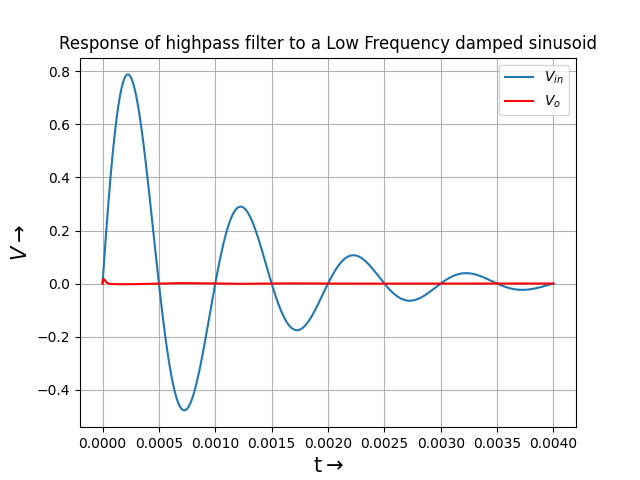
\includegraphics[scale=0.6]{Figure_7.png}
	\caption{Low frequency damped sinusoid}
	\label{fig:System Response with Decay = 0.05}
\end{figure}

The high pass filter responds by quickly attenuating the input. Notice that the time scales show that the high pass filter response is orders of magnitudes faster than the low pass response. This is because the input frequency is below the cutoff frequency, so the output goes to $0$ very fast.

\subsubsection{High frequency damped sinusoid}
The High frequency damping sinusoid is given by:
\begin{equation}
    f(t) = cos(10^7t)*e^{-3000t}
\end{equation}
It is expected that it will be fully attenuated by the Low passs filter while it will pass through the high pass filter with almost no change.
\begin{figure}[h!]
\centering
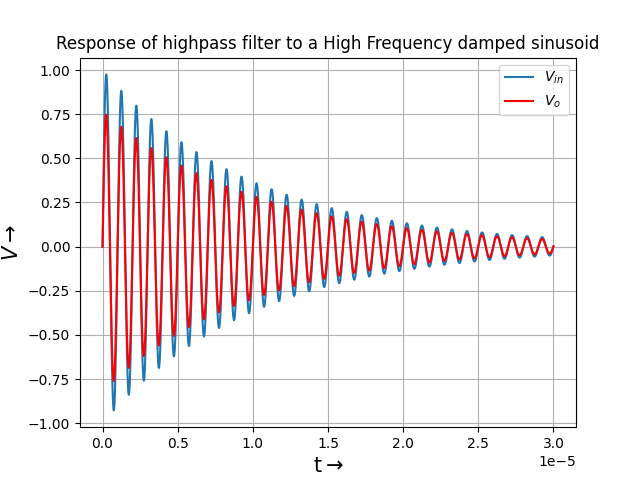
\includegraphics[scale=0.6]{Figure_8.png}
\caption{High frequency damped sinusoid}
\label{fig:System Response with Decay = 0.05}
\end{figure}



\subsection{Question 5}
The unit step response, as expected is high at t=0 when there is an abrupt change in the input. Since there is no other change at large time values outside the neighbourhood of 0, the Fourier transform of the unit step has high values near 0 frequency, which the high pass filter attenuates.

\begin{figure}[h!]
\centering
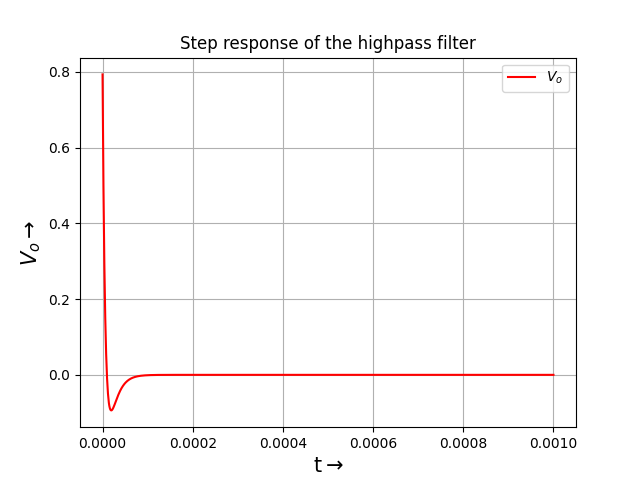
\includegraphics[scale=0.6]{Figure_9}
\caption{Step response of high pass filter}
\label{fig:System Response with Decay = 0.05}
\end{figure}

\section{Conclusion}


    In conclusion, the sympy module has allowed us to analyse quite complicated circuits by analytically solving their node equations. We then interpreted the solutions by plotting time domain responses using the signals toolbox. Thus, sympy combined with the scipy.signal module is a very useful toolbox for analyzing complicated systems like the active filters in this assignment.


\end{document}
